% ESE 6180 (Fall 2026) final-project proposal.
% Two pages maximum excluding references, L4DC (PMLR) format.
\documentclass{l4dc2026}

% amsmath, amssymb, natbib, graphicx, url, algorithm2e are loaded by the class.
\usepackage{times}

\title[Boundary-Guided Training of Closed-Loop Controllers]{From Evaluation to
Improvement: Boundary-Guided Training of Closed-Loop Controllers}

\author{%
 \Name{Shimin Chen} \Email{cshimin@engineering.upenn.edu}\\
 \addr Department of Electrical and Systems Engineering, University of Pennsylvania%
}

% Blank the proceedings banner ("Proceedings of Machine Learning Research vol
% vvv:1--N, 2026") that the class puts at the top of page 1. The class applies
% page style jmlrtps there via \maketitle, so append a head-clearing step to it
% rather than emptying \jmlryear, which would also drop the copyright footer.
\makeatletter
\g@addto@macro\ps@jmlrtps{\def\@oddhead{}\let\@evenhead\@oddhead}
\makeatother

\newcommand{\Zset}{\mathcal{Z}}

\begin{document}

\maketitle

\begin{abstract}%
A frozen controller's failures across operating conditions form a map of where it
works. We propose to investigate whether training near an estimated performance
boundary expands that region while limiting regression where the controller was
already acceptable. We certify the region of a frozen policy, feed that estimate
into the choice of training conditions, and re-certify on fresh data. Monotonic
improvement is the ambitious target, not an assumption.%
\end{abstract}

\section{Motivation, Problem Formulation, and Feedback Loops}

Evaluating a frozen controller across operating conditions maps where it works,
not just how well. On CartPole with the pole-angle cutoff relaxed to $90^\circ$,
call an episode a \emph{recovery} if it survives $500$ steps with final-100-step
RMS pole angle at most $5^\circ$. An adaptive sweep of initial pole angles and
half-lengths ($248$ conditions, $50$ seeds, $37{,}200$ episodes, no retraining)
gives Figure~\ref{fig:regions}: quantized LQR and PPO have recovery regions
differing in shape, not only size, and survival and recovery disagree, since
antisymmetrized PPO often survives from $\pm25^\circ$ without settling inside the
band. We ask whether evaluating that boundary can guide training that
\emph{expands} the acceptable region while limiting degradation elsewhere, which
signal---threshold proximity, intermediate difficulty, uncertainty, or
improvability---marks a useful training condition, and what assumptions permit a
guarantee. Informative \emph{evaluation} conditions need not be informative
\emph{training} conditions.

At iteration $k$, freeze $\pi_k$. For a condition $z\in\Zset$, horizon $H$, and
declared episode randomness $\xi\sim P_\xi(\cdot\mid z)$, let
$p_k(z)=\Pr_\xi[\tau_{\pi_k}(z,\xi)\text{ fails recovery}]$; under tolerance
$\alpha$ the acceptable region is $S_k=\{z:p_k(z)\le\alpha\}$. With a measure
$\mu$ fixed in advance, $V_k=\mu(S_k)$, $g_k=\mu(S_{k+1}\setminus S_k)$, and
$\ell_k=\mu(S_k\setminus S_{k+1})$ satisfy $V_{k+1}-V_k=g_k-\ell_k$. Three loops
nest---\textbf{control:} observation $\to$ action $\to$ next observation;
\textbf{evaluation:} condition selection $\to$ frozen rollout $\to$ updated
evidence $\to$ next condition; and \textbf{improvement}, studied here:
\[
\pi_k \;\longrightarrow\; \widehat{p}_k,\ \widehat{S}_k
      \;\longrightarrow\; q_k=(1-\lambda)q_{\mathrm{base}}+\lambda q_{\mathrm{target},k}
      \;\longrightarrow\; \mathrm{Train}(\pi_k,q_k)
      \;\longrightarrow\; \pi_{k+1}.
\]
Closing it moves the target from $p_k$ to $p_{k+1}$; policies change only in a
separate training phase, so each $\widehat{p}_k$ describes one closed-loop
system. What is distinctively L4DC is that the estimated quantity is a
closed-loop property of a learned controller over initial conditions and plant
parameters, not a reward, and that the object to certify and grow is a region,
not a scalar.

\begin{figure}[t]
\centering
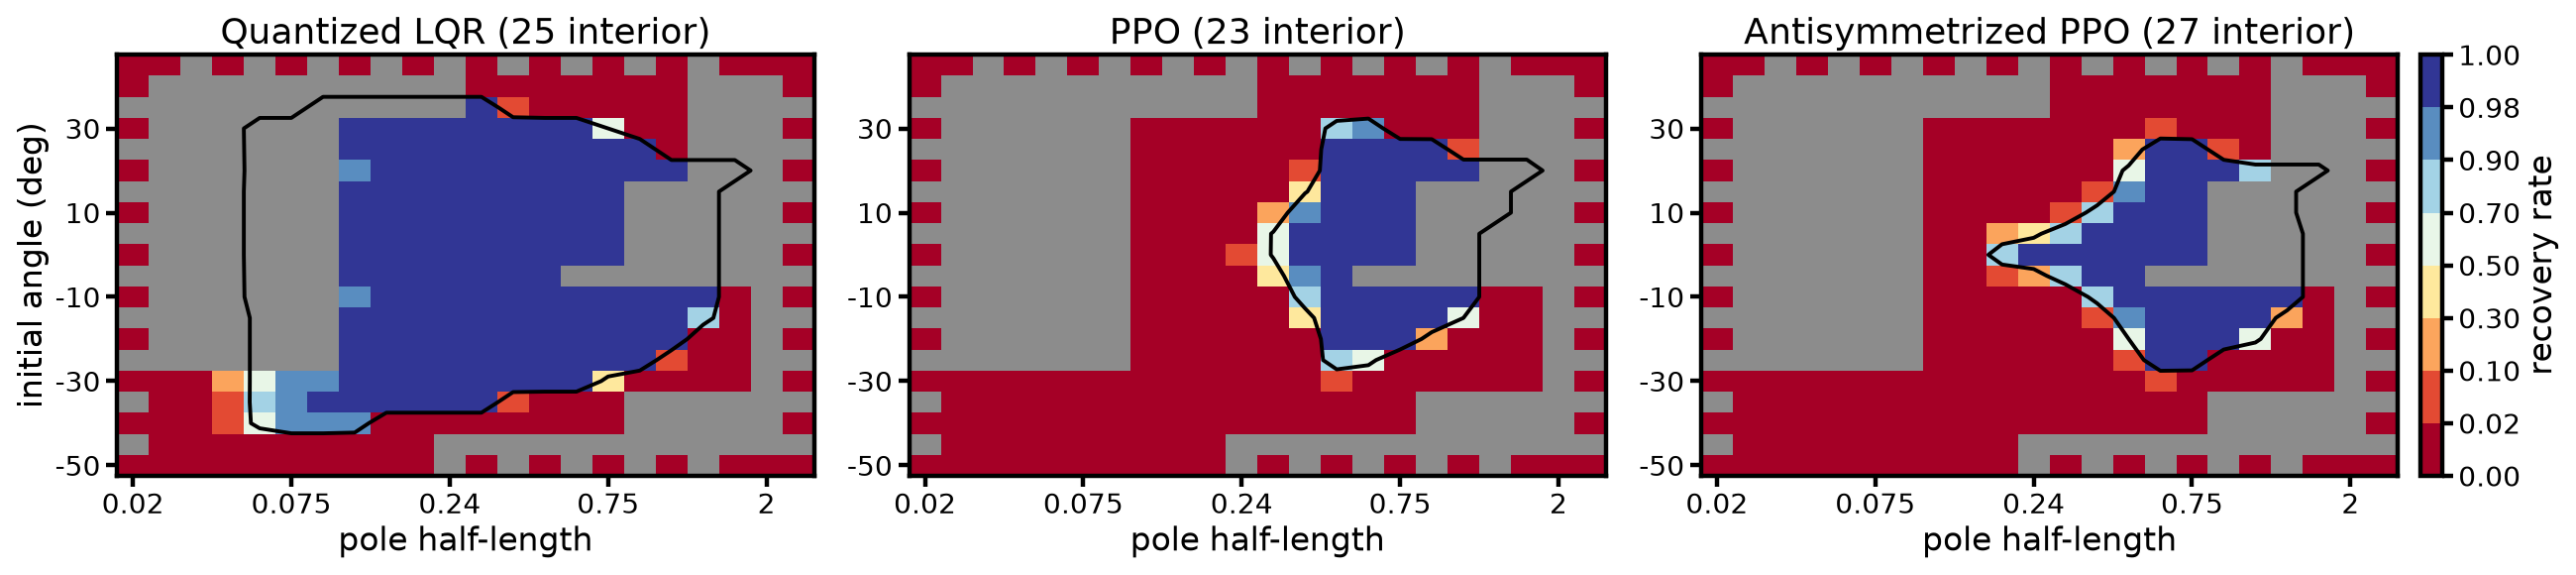
\includegraphics[width=0.76\textwidth]{figures/cartpole_recovery_regions.png}
\caption{Preliminary recovery rate for three \emph{frozen} controllers on the
angle/length lattice in mesh-rank coordinates ($248$ of $440$ slots sampled, gray
unsampled; black line is the $0.5$ contour). Over $92\%$ of cells are exactly $0$
or $1$: the interior cells are the whole boundary.}
\label{fig:regions}
\end{figure}

\section{Related Work}

\textbf{Evaluation.} \citet{gotovos2013active} and \citet{letham2022lookahead}
develop adaptive level-set estimation, the latter for Bernoulli observations like
ours; \citet{howard2021timeuniform} supply time-uniform confidence sequences, so
adaptive sampling still certifies. \textbf{Training-condition selection.} Reverse
curriculum generation \citep{florensa2017reverse} adapts start states to current
performance, prioritized level replay \citep{jiang2021prioritized} ranks
configurations by learning potential, and sampling for learnability
\citep{rutherford2024noregrets} targets mixed-success conditions, so
boundary-guided sampling is not itself novel; our contribution is the controlled
comparison under a fixed, certified protocol. \textbf{Control guarantees.}
\citet{berkenkamp2017safe} link model-based learning to safe-region expansion via
Lyapunov analysis; their stability certificates differ from our finite-horizon
recovery probabilities.

\section{Goals}

\textbf{Stage 1 (course foundation).} Build the evaluator: certify a condition
only when a confidence sequence puts its failure rate strictly on one side of
$\alpha$, and split $\sum_k\delta_k\le\delta$ so all certified sets hold with
probability $1-\delta$ (proved by Hoeffding and a union bound). For
$x_{j+1}=(A-BK)x_j$ and $J_{H,K}(x)=x^\top P_H(K)x$ on $\|x\|_2\le r$, the update
bound $|J_{H,K'}(x)-J_{H,K}(x)|\le r^2\|P_H(K')-P_H(K)\|_2=:b$ confines all
regression of the sublevel set $\{J_{H,K}\le h\}$ to the band $h-b<J_{H,K}\le h$.
These elementary results do not transfer automatically to the nonlinear learned
system.

\textbf{Stage 2 (main research).} From one frozen PPO checkpoint, branch into
matched training runs under three selection rules---uniform, boundary-guided over
a band at the estimated boundary, and intermediate-difficulty scored by
$\widehat{p}_k(1-\widehat{p}_k)$---holding $q_{\mathrm{base}}$, $\lambda$, the
objective, and the optimizer fixed. Starting with initial-angle variation, then
the angle--length domain of Figure~\ref{fig:regions}, we report $g_k$, $\ell_k$,
net coverage, maps of \emph{where} change occurs, seed variation, and total cost.
Each updated policy is re-certified on fresh data, separating certificate growth
from retraining. A negative result is a real outcome.

\textbf{Stage 3 (ambitious target).} Bound performance drift by update size,
horizon, and closed-loop amplification; construct examples where improving
selected conditions degrades others; and find a restricted controller class and
update admitting a sufficient condition for expansion. Both the continuous-cost
sublevel set and the level set $S_k$ are candidates. \textbf{Open decisions.}
Whether repeated rounds are required or a single $\pi_0\to\pi_1$ update suffices,
and which level-set notion is primary, stay open; $\alpha$, $\delta$, budgets,
seeds, reward, and mixture weights will be fixed and recorded beforehand.

\bibliography{../references}

\end{document}
